% Drawing 86/01-1 -- folder 86, batch 01, archive page 8 (PDF page 9).
% Transcription: figures : (C$_1$), au crayon et à l'encre, l'icosaèdre vu le long d'un axe passant par les milieux de deux arêtes opposées, sommets $u, v$, $u', v'$, $s, t$, $\Pi_{s,u}$, $\Pi_{t,v}$, … ; « ou » (C$_2$), la même vue en projection, sommets extérieurs $s'$, $u'$, $v'$, $t'$, points $\Pi_{t,u} = \Pi_{s',v'}$ (?), $\Pi_{t,v} = \Pi_{s',u'}$, $\Pi_{s,u} = \Pi_{t',v'}$, $\Pi_{s,v} = \Pi_{t',u'}$ ; (C$_3$), un schéma analogue plus petit, flèches vers $t'$ et $s'$
% Kind: icosahedron seen along an axis (three views). Method 2 (schematic redraw from the facsimile). Status: partial.
% Notes: (C1) the icosahedron seen along the axis through the midpoints of two opposite edges: outline with the four Pi vertices at the corners, u and v at the sides, the two inner vertices (t above, s below) joined to them; the dashed back edges are only indicated (u - v and one diagonal). (C2) the same in projection: circle, two nested squares, the horizontal and vertical axes, arrows to t' (up) and s' (down), and the four Pi labels with their equalities as the transcription reads them; the left outer label is read u' on the facsimile, the transcription has v' among the outer vertices (left as v', a reading). (C3) the smaller analogous scheme (a bipyramid over a small square) with arrows towards t' and s'. The pencil doublings are reduced to one stroke. "ou" between C1 and C2 is drawn; the labels (C1), (C2) are placed as on the page. Not encoded: the three views are projections whose hidden edges are not all drawn.
% Coordinates: 1 unit = 1 mm = 1/100 of the crop width (bbox in page fractions: [0.12, 0.4, 0.92, 0.68]).
% Redrawn by Claude (claude-opus-5-5), issue #73, 2026-11-07; not checked by a human; not compiled (no TeX in the session).
% Rights: reproduces part of the work -- behind RENDER_TRANSCRIPTS, never published by itself.
\documentclass[tikz,border=3pt]{standalone}
\usepackage{amsmath,amssymb}
\usetikzlibrary{patterns,arrows.meta}
\tikzset{pencil/.style={black!45}, struck/.style={black!35}, mark/.style={circle,draw,inner sep=1.3pt}, pt/.style={circle,fill,inner sep=0.9pt}, opt/.style={circle,draw,fill=white,inner sep=1.1pt}}
\begin{document}
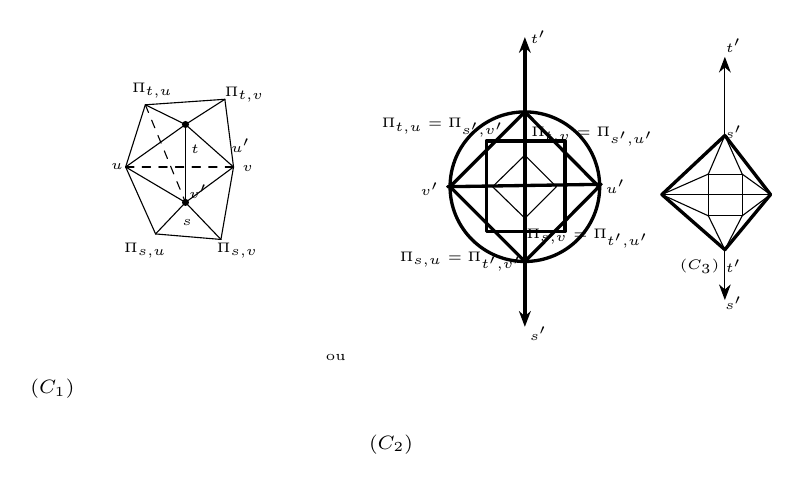
\begin{tikzpicture}[x=1mm,y=1mm,line cap=round,line join=round,font=\scriptsize]
\draw (16.8,-14.9) -- (26.9,-14.2);
\draw (26.9,-14.2) -- (28,-22.8);
\draw (28,-22.8) -- (26.4,-32);
\draw (26.4,-32) -- (18.1,-31.3);
\draw (18.1,-31.3) -- (14.3,-22.8);
\draw (14.3,-22.8) -- (16.8,-14.9);
\draw (21.9,-17.4) -- (16.8,-14.9);
\draw (21.9,-17.4) -- (26.9,-14.2);
\draw (21.9,-17.4) -- (14.3,-22.8);
\draw (21.9,-17.4) -- (28,-22.8);
\draw (21.9,-27.3) -- (18.1,-31.3);
\draw (21.9,-27.3) -- (26.4,-32);
\draw (21.9,-27.3) -- (14.3,-22.8);
\draw (21.9,-27.3) -- (28,-22.8);
\draw (21.9,-17.4) -- (21.9,-27.3);
\draw[dashed] (14.3,-22.8) -- (28,-22.8);
\draw[dashed] (16.8,-14.9) -- (21.9,-27.3);
\node[pt] at (21.9,-17.4) {};
\node[pt] at (21.9,-27.3) {};
\node[inner sep=1pt] at (17.7,-13.1) {\tiny $\Pi_{t,u}$};
\node[inner sep=1pt] at (29.4,-13.6) {\tiny $\Pi_{t,v}$};
\node[inner sep=1pt] at (16.8,-33.4) {\tiny $\Pi_{s,u}$};
\node[inner sep=1pt] at (28.5,-33.4) {\tiny $\Pi_{s,v}$};
\node[inner sep=1pt] at (13.2,-22.8) {\tiny $u$};
\node[inner sep=1pt] at (29.8,-23) {\tiny $v$};
\node[inner sep=1pt] at (23.1,-20.5) {\tiny $t$};
\node[inner sep=1pt] at (22.1,-29.8) {\tiny $s$};
\node[inner sep=1pt] at (28.9,-20.1) {\tiny $u'$};
\node[inner sep=1pt] at (23.5,-25.9) {\tiny $v'$};
\draw[very thick] (65,-25.3) circle[radius=9.5];
\draw[very thick] (60.1,-19.5) -- (70.1,-19.5) -- (70.1,-31) -- (60.1,-31) -- cycle;
\draw[very thick] (65,-15.8) -- (74.4,-25.3) -- (65,-34.8) -- (55.5,-25.3) -- cycle;
\draw (65,-21.3) -- (69,-25.3) -- (65,-29.3) -- (60.9,-25.3) -- cycle;
\draw[very thick] (55.2,-25.3) -- (74.7,-25);
\draw[very thick] (65,-15.8) -- (65,-34.8);
\draw[-{Stealth[length=2mm]},very thick] (65,-15.8) -- (65,-6.3);
\draw[-{Stealth[length=2mm]},very thick] (65,-34.8) -- (65,-43.1);
\node[inner sep=1pt] at (66.7,-6.3) {\tiny $t'$};
\node[inner sep=1pt] at (66.7,-44) {\tiny $s'$};
\node[inner sep=1pt] at (76.5,-25.3) {\tiny $u'$};
\node[inner sep=1pt] at (52.9,-25.6) {\tiny $v'$};
\node[inner sep=1pt] at (54.6,-17.8) {\tiny $\Pi_{t,u}=\Pi_{s',v'}$};
\node[inner sep=1pt] at (73.6,-19) {\tiny $\Pi_{t,v}=\Pi_{s',u'}$};
\node[inner sep=1pt] at (56.9,-34.8) {\tiny $\Pi_{s,u}=\Pi_{t',v'}$};
\node[inner sep=1pt] at (73,-31.9) {\tiny $\Pi_{s,v}=\Pi_{t',u'}$};
\draw[very thick] (90.4,-18.8) -- (82.4,-26.3) -- (90.4,-33.3) -- (96.2,-26.3) -- cycle;
\draw (88.3,-23.7) -- (92.6,-23.7) -- (92.6,-29) -- (88.3,-29) -- cycle;
\draw (90.4,-18.8) -- (88.3,-23.7);
\draw (90.4,-18.8) -- (92.6,-23.7);
\draw (90.4,-33.3) -- (92.6,-29);
\draw (90.4,-33.3) -- (88.3,-29);
\draw (82.4,-26.3) -- (88.3,-23.7);
\draw (82.4,-26.3) -- (88.3,-29);
\draw (96.2,-26.3) -- (92.6,-23.7);
\draw (96.2,-26.3) -- (92.6,-29);
\draw (82.4,-26.3) -- (96.2,-26.3);
\draw[-{Stealth[length=2mm]}] (90.4,-18.8) -- (90.4,-8.8);
\draw[-{Stealth[length=2mm]}] (90.4,-33.3) -- (90.4,-39.7);
\node[inner sep=1pt] at (91.5,-7.4) {\tiny $t'$};
\node[inner sep=1pt] at (91.5,-40.1) {\tiny $s'$};
\node[inner sep=1pt] at (91.5,-18.4) {\tiny $s'$};
\node[inner sep=1pt] at (91.5,-35.4) {\tiny $t'$};
\node[inner sep=1pt] at (87.2,-35.4) {\tiny $(C_3)$};
\node[inner sep=1pt] at (5,-51) {\scriptsize $(C_1)$};
\node[inner sep=1pt] at (41,-47) {\tiny ou};
\node[inner sep=1pt] at (48,-58) {\scriptsize $(C_2)$};
\end{tikzpicture}
\end{document}
